\chapter{绪论}

\section{研究背景与研究意义}
\label{sec:research_background}
和去年巴西大停电联系一下

\section{国内外研究现状}
\label{sec:research_presentSituation}

\subsection{脆弱性研究起源及现状}
\label{sec:origin}


\subsection{电力系统脆弱性研究综述}
\label{sec:presentPowerSys}


\subsection{电力系统脆弱性量化评估研究现状}
\label{sec:presentSituation3}

\section{研究内容与研究路线}
\label{sec:research_curise}

\subsection{待解决的问题}
\label{sec:research_problem}
对于电力系统的脆弱性分析与量化评估的研究至今依然存在很多待解决的问题,如:
\begin{enumerate}[(1)]
  \item 脆弱性概念虽然很早就已经提出,但对于电力系统的脆弱性描述尚不清晰,缺乏全面性;
  \item 电力系统中的脆弱性研究的研究理论与方法虽然比较权威和可行,但是在脆弱性指标研究方面却考虑的不够全面;
  \item 在指标融合方法上,虽然各个领域的指标融合方法各有千秋,但对于在电力系统的指标融合方面的考虑不够合理全面;
  \item 对于电力系统脆弱性量化分析与研究,脆弱性量化分析模型的相关研究未形成严格的理论体系。
 \end{enumerate}

\subsection{研究内容与章节划分}
\label{sec:contendAndIdea}
本文针对含风电电力系统脆弱性分析与量化研究中待解决的问题,在研究了系统的特性与模型的基础上,给出了较为科学的含风电电力系统脆弱性定义。针对定义分别从系统结构与系统状态两方面进行脆弱性理论分析。根据结构脆弱性和状态脆弱性的理论研究进行脆弱性指标选取,从而建立系统脆弱性综合评估指标集。分别对一级脆弱性指标和二级脆弱性指标进行量化、权重分配、指标融合形成了含风电电力系统脆弱性量化模型。并且以$IEEE39$系统数据为例进行含风电电力系统的脆弱性分析与量化,识别系统的薄弱环节。本文的章节安排如下:

第~1~章~:查阅国内外“风力发电”、“脆弱性分析”等相关领域研究文献与论文,对脆弱性概念的起源与发展以及脆弱性在电力系统的研究现状做了详细的调研与综述,为后续研究含风电电力系统脆弱性与量化分析方法提供必要的理论依据。在明确研究对象的基础上,科学提炼出待解决的问题,确定研究方法、目标和技术路线;

第~2~章~:

第~3~章~:通过研究含风电电力系统自身存在脆弱性的原因,得出系统脆弱性的本质和系统脆弱性的数学描述,在此基础上,结合前人的研究,得到了含风电电力系统的脆弱性的定义。分别从系统的结构和系统的状态两个角度对脆弱性进行分析研究。结构脆弱性从系统拓扑的角度,研究了系统在运行中,保持其拓扑完整性的能力。而状态脆弱性则专注研究外界环境的变化使系统暴露出的缺陷,即向坏的方向发展的趋势;

第~4~章~:针对结构脆弱性与状态脆弱性,分别根据各自脆弱性的定义与特征选取能够反映其脆弱现象的评价指标,结合综合评价法及多指标融合法,建立了系统脆弱性量化评估的数学模型。解决了系统脆弱性现象难以量化的问题,为后续分析含风电电力系统脆弱性问题奠定了理论基础;

第~5~章~:以$IEEE39$电力系统为例,在系统模型建立的基础上,分别研究了单风机接入和多风机接入下系统的脆弱性。单风机接入的情况下,研究了系统的结构脆弱性,并且对比了不同风机接入下系统的状态脆弱性,最终得到单风机系统的综合脆弱性。多风机接入的情况下,首先对比了双风机与单风机系统的脆弱性,再对多风机系统的脆弱性进行分析。最后,使用不同的电力系统数据进行脆弱性量化分析;

第~6~章~:总结本文的研究工作,对本文中电力系统脆弱性分析与量化数学模型的优点和不足进行了详细的阐述,并为后续研究工作提出了若干点建议与展望。

通过以上的研究工作,完成电力系统脆弱性分析与量化评估的理论研究及实验验证与分析,具体的技术路线图如下所示。
\begin{figure}[H] % use float package if you want it here
  \centering
  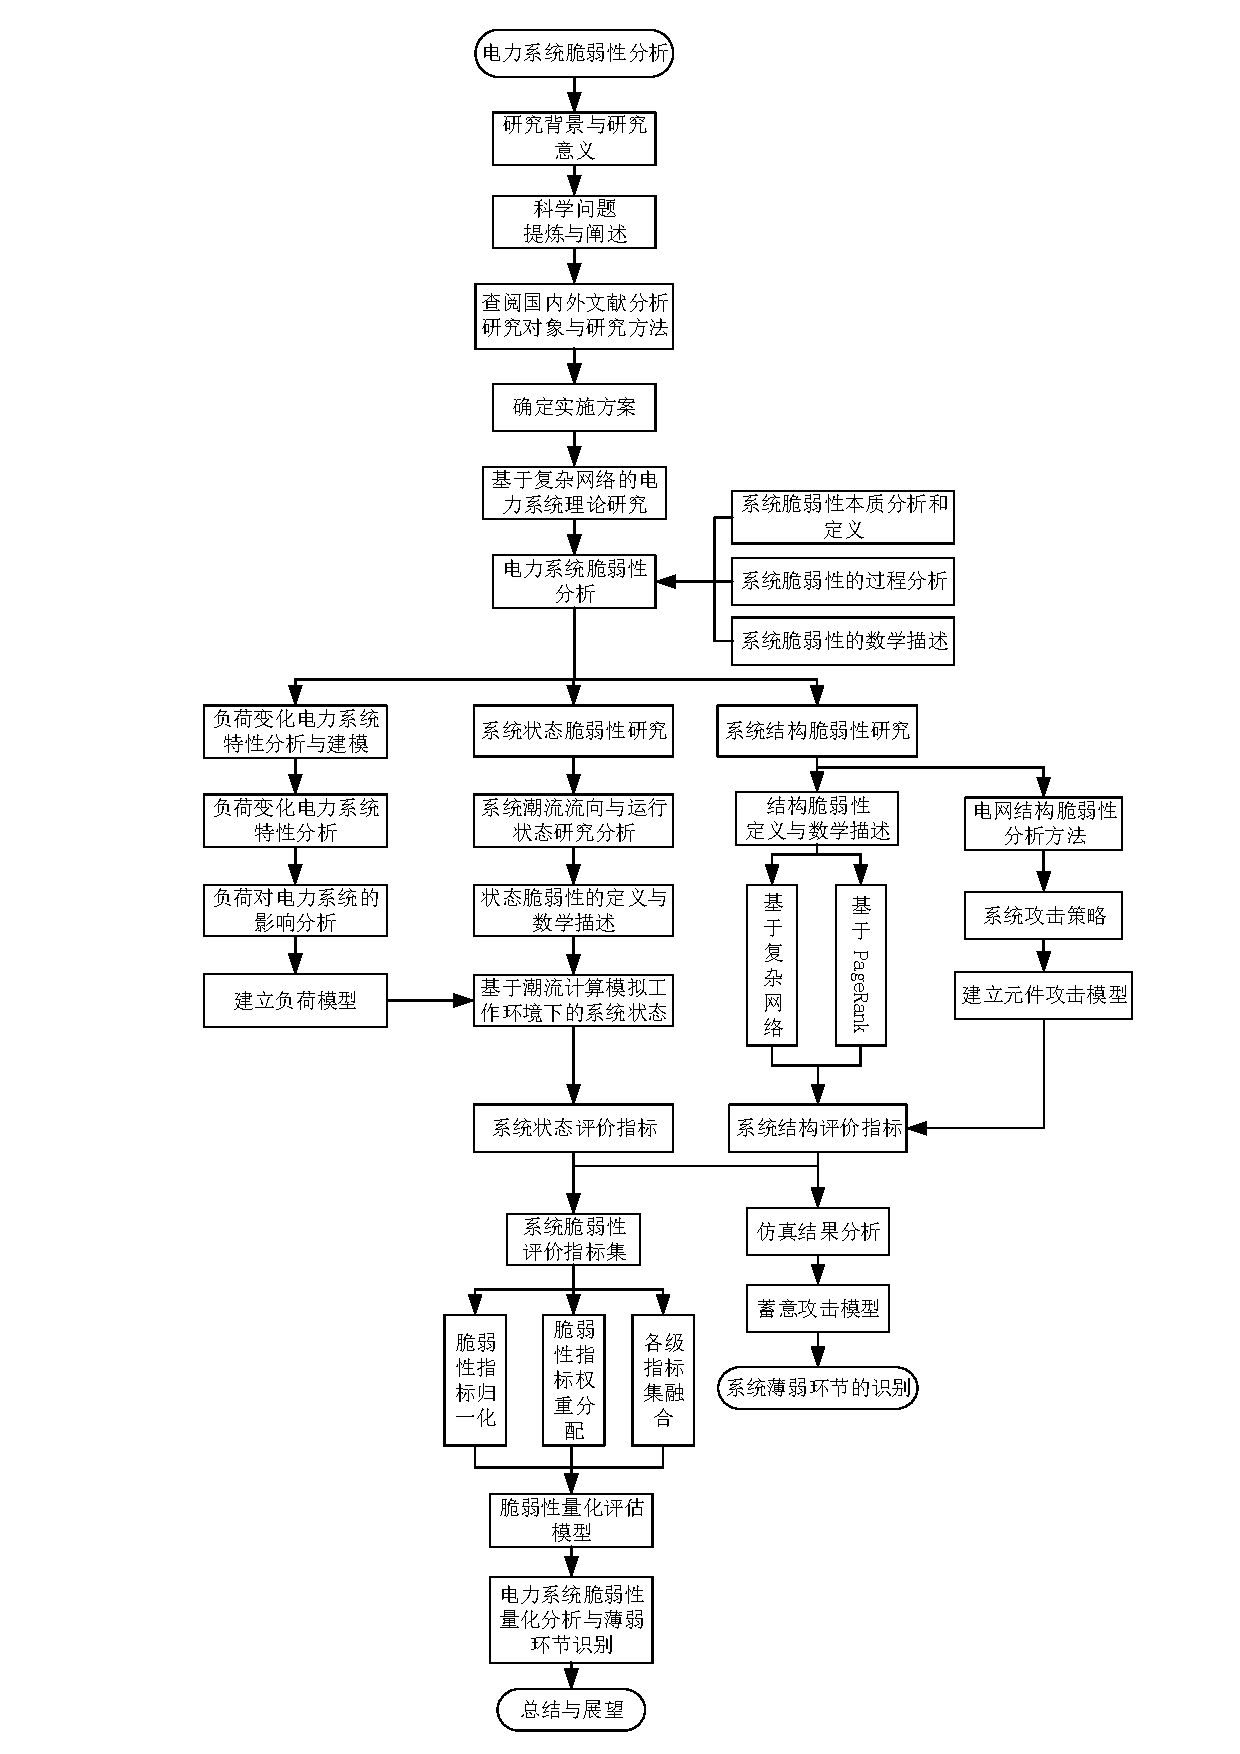
\includegraphics[height=23cm]{technicalRoute.pdf}
  \caption{技术路线图}
  \label{fig:technicalRoute}
\end{figure}
